% =============================================================================
% Rethinking RUL Labeling Strategies in Bearing Prognostics:
% Converged Multi-Dataset Evidence for Evaluation Inflation
% v5 response to second review
% =============================================================================
\documentclass[5p,twocolumn]{elsarticle}

\usepackage[utf8]{inputenc}
\usepackage{amsmath,amssymb}
\usepackage{graphicx}
\usepackage{booktabs}
\usepackage{hyperref}
\usepackage{bm}
\usepackage{float}
\usepackage{multirow}

\journal{Measurement}

\graphicspath{{figures/}}

\begin{document}

\begin{frontmatter}

\title{Revisiting Evaluation Protocols for Bearing Remaining Useful Life Prediction: A Multi-Dataset Study of Labeling and Temporal Split Effects}

\author[1]{Zhongkuan Ma\corref{cor1}}
\ead{2024212760@nefu.edu.cn}
\cortext[cor1]{Corresponding author. ORCID: 0009-0003-4491-6619}

\begin{abstract}
Recent bearing RUL studies often report high $R^2$ values under diverse evaluation protocols. Two protocol choices examined in this study are piecewise linear labels with an 80\% plateau and random time-step splitting. We evaluate these choices under converged training on three public datasets (XJTU-SY, PHM2012, IMS) with Linear Regression, LSTM, TCN, PatchTST, a constant predictor baseline, leave-one-bearing-out cross-validation (LOOCV), and three-seed random time-step splits. On XJTU-SY, piecewise labels increase LOOCV $R^2$ by $0.20$--$0.23$, while random splitting adds little. On PHM2012 and IMS, random splitting raises $R^2$ from negative values or $0.17$--$0.25$ under linear LOOCV to $0.70$--$0.86$ under piecewise random splitting, especially on datasets with stronger cross-bearing distribution shifts. The reproduced protocol family shows large protocol-induced inflation, but it does not reach the $R^2>0.99$ magnitude of any specific publication. In all twelve model-dataset cells, every piecewise random-split run exceeded every linear-LOOCV fold (Cliff's delta $=1.0$). Reported high scores in this protocol family are consistent with within-trajectory dependence and interpolation, but they do not prove that every published near-perfect result is caused by the protocol. We report per-fold results, 95\% confidence intervals, effect sizes, RMSE, MAE, split-ratio sensitivity, and convergence epochs, and we summarize the findings into a four-component STAR reporting template: continuous labels, leave-one-bearing-out cross-validation, constant baselines, and multi-model reporting.
\end{abstract}

\begin{keyword}
RUL Prediction \sep Bearing Prognostics \sep Evaluation Methodology \sep Labeling Bias \sep Temporal Splitting \sep Reproducibility
\end{keyword}

\end{frontmatter}

\section{Introduction}
Rolling bearings are critical components in rotating machinery, and accurate prediction of their remaining useful life (RUL) supports maintenance scheduling and failure prevention. In recent years, deep learning methods have reported high $R^2$ values on public bearing datasets \cite{rul_lstm_uq_2022,reg_lstm_2021,gru_tim_2021,transformer_tim_2023}. Most of these studies share two evaluation practices: piecewise linear labels with an 80\% plateau and random splitting of sliding-window samples across the full life trajectory.
In practical manufacturing systems, RUL models are expected to generalize across different assets rather than interpolate previously observed degradation trajectories. These choices are not merely reporting details; they define different prediction tasks. A piecewise label with an 80\% plateau holds most of a trajectory at one target value, which turns much of the regression into a transition-detection problem. A random split of sliding windows can put temporally adjacent samples from the same bearing on both sides of the training/test boundary, which makes the test task an interpolation on a trajectory the model has already seen. When both choices appear together, a benchmark can report high performance without showing whether the model predicts degradation for a new bearing. This study separates those two effects empirically.

A previous version of this study used a fast five-epoch protocol on XJTU-SY only. That protocol was insufficient for comparison with published models trained to convergence. This revision replaces that protocol with converged training, adds PHM2012 and IMS, and reports split-ratio sensitivity.

We contribute:
\begin{enumerate}
    \item a converged comparison of linear and piecewise labels under LOOCV and random time-step splitting on XJTU-SY, PHM2012, and IMS;
    \item per-fold results, 95\% confidence intervals, bounded effect sizes, RMSE, and MAE for all model-dataset combinations;
    \item protocol-level reproduction of the inflation phenomenon associated with the dominant evaluation design, with explicit caveats about the reproduced $R^2$ range;
    \item random split-ratio and chronological time-block sensitivity analysis;
\item an auditable STAR evaluation template with continuous labels, per-bearing holdout, constant baselines, and multi-model reporting.
\end{enumerate}

\section{Motivating Protocol Choices}
Recent bearing RUL studies frequently combine piecewise linear labels with an 80\% plateau and random time-step splitting. We do not report a quantitative literature survey in this version. Instead, we directly evaluate these two protocol choices under controlled experiments on three public datasets, so the claims remain auditable through the reported results and reproducibility package.

A prevalence count would require access to the full methods and code of each surveyed paper. Those details are often incomplete, so a controlled comparison on public data offers a more direct test of the protocol effect. The same preprocessing, models, seeds, and metrics are used for every protocol in this study. Differences in $R^2$ can therefore be attributed to the protocol rather than to implementation choices.

\section{Related Work}
Bearing RUL prediction has moved from physics-based degradation models to data-driven models built on CNNs, recurrent networks, and transformers \cite{rul_lstm_uq_2022,reg_lstm_2021,transformer_tim_2023}. Much of this literature concentrates on architecture design. Evaluation protocols receive less attention, and reviews note the absence of standardized benchmarks \cite{zhao2021deep,caesarendra2021machine}.

Label construction is usually treated as fixed preprocessing, but it changes the difficulty of the target. A plateau at the start of life compresses most of the label distribution into a single value. The effect of this compression depends on the dataset and the split, which is why label and split should be evaluated jointly rather than in isolation.

Recent time-series and ecological studies distinguish direct sample leakage from within-trajectory dependence \cite{leakage_nature,leakage_frontiers}. The distinction matters for this paper. Random splitting does not copy identical samples into training and test. It places dependent samples from the same trajectory on both sides of the split, so the test task becomes interpolation-friendly evaluation. We use that terminology rather than describing the protocol as invalid.

The methodological gap is whether reported scores measure prediction for new bearings or interpolation within the same bearing. Our study measures both on the same preprocessing, models, seeds, and metrics.

We do not include a paper-level protocol table in this version. In many studies, the split and label details are not reported at a level that allows reliable classification from metadata or abstracts. A table built from incomplete information would introduce the same reproducibility problem this paper addresses. The protocol choices used here are instead grounded in the two practices discussed in the cited RUL and time-series evaluation literature.

\subsection{Evaluation Protocols in Prognostics}
Time-series evaluation protocols differ in what they ask a model to do. A random split of sliding windows keeps samples from the same trajectory on both sides of the training/test boundary. The test task then becomes interpolation on a trajectory the model has already observed. A chronological split keeps the same bearing in training but asks the model to extrapolate into later degradation stages. A grouped-by-bearing split removes the test bearing from training and therefore measures new-bearing generalization. These protocols are not interchangeable, and reported performance cannot be compared across them without specifying which task was used.

Bearing run-to-failure signals add another complication. Consecutive windows are strongly autocorrelated, and the degradation process is monotonic in most cases. A model trained on random windows from the same bearing can memorize the trajectory shape and use nearby temporal context to interpolate test samples. That behavior is useful for tracking a known degradation process, but it is not evidence that the model can predict the behavior of a new bearing under a different load or operating condition.

The same issue appears in other time-series domains, where direct sample leakage is distinguished from dependence-induced interpolation \cite{leakage_nature,leakage_frontiers}. For bearing RUL, the practical consequence is that benchmark scores should be interpreted as properties of the joint choice of label and split, not as standalone properties of the model. The STAR checklist proposed later makes this dependency explicit.

\section{Methodology}
\subsection{Datasets}
We use three public run-to-failure datasets:
\begin{itemize}
    \item \textbf{XJTU-SY} \cite{xjtusy2019dataset}: 8 run-to-failure bearings (Bearing1\_1 through Bearing1\_5 and Bearing2\_1 through Bearing2\_3) from conditions 1 and 2, yielding 15,928 windows.
    \item \textbf{PHM2012} \cite{nectoux2012pronostia}: 6 learning-set bearings, yielding 7,534 windows.
    \item \textbf{IMS} \cite{ims2006}: 3 run-to-failure test sets (first, second, and fourth), yielding 75,712 windows.
\end{itemize}
The PU dataset is a benchmark for fault classification rather than full run-to-failure RUL trajectories, so it is not used for RUL label generation. Each vibration signal is segmented into non-overlapping windows of 2,560 samples; the stride therefore equals the window length. Ten statistical and spectral features are extracted per window, and a history length of 10 windows is used for LSTM, TCN, and PatchTST inputs. History sequences are constructed within each bearing before splitting, so a random split can place temporally adjacent sequences from the same trajectory in both training and test sets; cross-bearing LOOCV avoids this overlap by construction. Feature normalization parameters are estimated from the training split only and applied to validation and test splits.

RUL labels are normalized to the $[0,1]$ range within each trajectory. This removes differences in absolute life span across datasets and keeps the regression target comparable. PHM2012 is used with its six learning-set bearings because the public challenge test set does not provide ground-truth RUL for supervised cross-validation.

\subsection{Labels and Evaluation Protocols}
We compare two label families:
\begin{equation}
\text{RUL}_{\text{lin}}(t) = 1 - t/T,
\label{eq:linear}
\end{equation}
\begin{equation}
\text{RUL}_{\text{pw}}(t) =
\begin{cases}
1.0, & t < 0.8T \\
(T - t)/(0.2T), & t \geq 0.8T.
\end{cases}
\label{eq:piecewise}
\end{equation}

The primary cross-bearing evaluation protocol is linear labels with leave-one-bearing-out cross-validation (LOOCV). For each test bearing, one other bearing is used for validation, and the remaining bearings are used for training. The dominant published protocol is reproduced as piecewise labels with a 70\%/15\%/15\% random time-step split over all windows.

\begin{figure}[t]
\centering
\fbox{\parbox{0.95\textwidth}{%
\small
\textbf{LOOCV:} train on bearings A and B, validate on bearing C, test on bearing D. No window from D appears in training or validation.\\
\textbf{Random split:} all windows from A, B, C, and D are pooled and randomly divided into train, validation, and test sets. Adjacent windows from the same trajectory can fall on different sides of the split.\\
\textbf{Chronological split:} for each bearing, the first 70\% of windows are used for training, the next 15\% for validation, and the last 15\% for testing.
}}
\caption{Comparison of the three evaluation protocols used in this study.}
\label{fig:protocols}
\end{figure}

\subsection{Models and Training}
We use four learned model classes:
\begin{itemize}
    \item \textbf{Linear Regression} on the 10 extracted features;
    \item \textbf{LSTM}: two-layer LSTM with 128 hidden units;
    \item \textbf{TCN}: dilated temporal convolutional network with channel widths $32 \to 64 \to 128$.
    \item \textbf{PatchTST} \cite{patchtst2023}: patch-based time-series transformer with patch length 4, stride 2, embedding dimension 64, four attention heads, and three encoder layers.
\end{itemize}
A constant predictor baseline, which always outputs the mean training RUL, is reported as the reference floor.

The models are treated as model classes with different inductive biases, not as state-of-the-art contestants. Hyperparameters are fixed before the protocol comparison. The LSTM uses two layers of 128 units. The TCN uses kernel size 3, dropout 0.2, hidden dimension 64, and channel widths 32, 64, and 128. PatchTST uses patch length 4, stride 2, embedding dimension 64, four attention heads, three encoder layers, and dropout 0.1.

CNN-based models are not included because this study focuses on protocol sensitivity rather than architecture ranking. The selected models cover linear, recurrent, convolutional temporal, and transformer-based inductive biases, which is sufficient to test whether the protocol effect survives across different model families.

All neural models are trained with MSE loss, AdamW, cosine annealing, batch size 1024, and early stopping with patience 30. XJTU-SY and PHM2012 use a maximum of 100 epochs; IMS uses a maximum of 60 epochs because of its much larger size. The best validation epoch is recorded for every run. The mean best epochs range from 2 to 97 across model-dataset combinations, confirming that the protocol allows convergence or early-stopping where cross-bearing generalization fails.

\subsection{Statistical Reporting}
For LOOCV, we report the mean $R^2$, standard deviation, and 95\% confidence interval computed with Student's $t$-distribution across held-out bearings. The CI reflects between-bearing fold variance, not sample-level prediction variance. Per-fold values are stored in the reproducibility artifacts.

Two points about these intervals should be stated. On XJTU-SY, the held-out bearings are similar in window count and degradation structure, and the same six training bearings are used in every fold except for the rotating validation bearing. Fold-level $R^2$ is therefore highly consistent and the CI is narrow. On IMS, only three test sets exist, so the CI is wide; IMS should be interpreted as directional evidence rather than a precise estimate.

Random splitting is repeated with three fixed seeds; we report the mean and the observed min--max range. Effect sizes are reported with Cliff's delta:
\begin{equation}
\delta = \frac{\#(x_i > y_j) - \#(x_i < y_j)}{n_x n_y},
\label{eq:cliff}
\end{equation}
where one distribution is compared with the other element-wise. Cliff's delta is bounded in $[-1, 1]$ and avoids the distortion of Cohen's $d$ when fold-level variance is tiny.

\subsection{Split Sensitivity Analysis}
To check whether the random-split result depends on the specific 70/15/15 ratio, we add two additional random ratios with TCN and piecewise labels:
\begin{itemize}
    \item 60\%/20\%/20\%;
    \item 80\%/10\%/10\%.
\end{itemize}
We also implement a chronological time-block split at 70\%/15\%/15\%: each bearing trajectory is split by time, with the first 70\% of windows used for training, the next 15\% for validation, and the final 15\% for testing. This removes random interleaving while still training on the same bearing as the test set. Chronological evaluation also involves temporal extrapolation and degradation-stage imbalance, so the negative $R^2$ values should be interpreted as a combination of these factors rather than as a pure leakage measurement.

\section{Results}
\subsection{Main Results}
Table~\ref{tab:main} summarizes the three datasets. The key pattern is that piecewise labels alone are not the universal source of inflation. On XJTU-SY, piecewise labels improve LOOCV $R^2$ by $0.20$--$0.23$ for every model, and random splitting adds no more than $0.02$. On PHM2012 and IMS, piecewise LOOCV often performs worse than linear LOOCV or below the constant baseline. The dominant inflation on those datasets is random time-step splitting.

For example, PHM2012 TCN obtains $0.174$ under linear LOOCV and $-0.260$ under piecewise LOOCV, but $0.862$ under piecewise random splitting. IMS TCN obtains $-2.331$ under linear LOOCV and $0.715$ under piecewise random splitting. PatchTST shows the same pattern: PHM2012 moves from $0.369$ under linear LOOCV to $0.850$ under piecewise random splitting, and IMS moves from $-1.058$ to $0.681$. Across all twelve model-dataset cells, every piecewise random-split run exceeds every linear-LOOCV fold, giving Cliff's delta $=1.0$ for the protocol effect.

\begin{table*}[t]
\centering
\caption{Converged protocol comparison. LOOCV $R^2$ values are mean [95\% CI]; random values are mean [min--max] across three seeds. $\delta_{\text{label}}$ compares piecewise LOOCV with linear LOOCV folds; $\delta_{\text{protocol}}$ compares piecewise random runs with linear LOOCV folds.}
\label{tab:main}
\small
\resizebox{\textwidth}{!}{%
\begin{tabular}{llccccccl}
\toprule
Dataset & Model & Linear LOOCV & Piecewise LOOCV & $\Delta$ label & Piecewise random & $\Delta$ protocol & $\delta_{\text{label}}$ & $\delta_{\text{protocol}}$ \\
\midrule
XJTU-SY & Linear Reg. & 0.178 [0.176; 0.180] & 0.410 [0.410; 0.411] & 0.232 & 0.430 [0.414; 0.447] & 0.252 & 1.000 & 1.000 \\
 & LSTM & 0.223 [0.221; 0.224] & 0.422 [0.422; 0.423] & 0.200 & 0.422 [0.401; 0.435] & 0.199 & 1.000 & 1.000 \\
 & TCN & 0.222 [0.220; 0.224] & 0.428 [0.427; 0.428] & 0.206 & 0.421 [0.396; 0.433] & 0.199 & 1.000 & 1.000 \\
 & PatchTST & 0.222 [0.220; 0.224] & 0.429 [0.428; 0.430] & 0.207 & 0.439 [0.425; 0.453] & 0.217 & 1.000 & 1.000 \\
\midrule
PHM2012 & Linear Reg. & $-0.168$ [$-0.366$; 0.029] & $-0.256$ [$-1.058$; 0.546] & $-0.088$ & 0.397 [0.376; 0.420] & 0.566 & 0.111 & 1.000 \\
 & LSTM & 0.245 [0.020; 0.469] & $-0.896$ [$-2.668$; 0.875] & $-1.141$ & 0.791 [0.778; 0.803] & 0.546 & $-0.389$ & 1.000 \\
 & TCN & 0.174 [0.030; 0.318] & $-0.260$ [$-1.153$; 0.633] & $-0.434$ & 0.862 [0.859; 0.865] & 0.688 & $-0.333$ & 1.000 \\
 & PatchTST & 0.369 [0.159; 0.578] & $-0.530$ [$-1.968$; 0.909] & $-0.899$ & 0.850 [0.841; 0.855] & 0.481 & $-0.611$ & 1.000 \\
\midrule
IMS & Linear Reg. & $-2.109$ [$-5.677$; 1.459] & $-4.586$ [$-25.477$; 16.305] & $-2.477$ & 0.320 [0.313; 0.328] & 2.429 & 0.333 & 1.000 \\
 & LSTM & $-1.208$ [$-3.714$; 1.297] & $-0.886$ [$-3.590$; 1.818] & 0.322 & 0.699 [0.695; 0.706] & 1.907 & 0.556 & 1.000 \\
 & TCN & $-2.331$ [$-5.216$; 0.554] & $-0.302$ [$-1.257$; 0.653] & 2.029 & 0.715 [0.714; 0.717] & 3.046 & 1.000 & 1.000 \\
 & PatchTST & $-1.058$ [$-3.125$; 1.009] & $-2.799$ [$-9.452$; 3.855] & $-1.741$ & 0.681 [0.674; 0.689] & 1.739 & $-0.556$ & 1.000 \\
\bottomrule
\end{tabular}}
\end{table*}

Because $R^2$ can be negative and is less interpretable under severe cross-bearing distribution shift, Table~\ref{tab:errors} additionally reports RMSE and MAE for the primary cross-bearing protocol (linear labels, LOOCV) and the reproduced dominant protocol (piecewise labels, random split). These absolute-error metrics confirm the same direction as the $R^2$ results: the protocol change substantially reduces prediction error even when the LOOCV $R^2$ is negative.

Table~\ref{tab:factorial} reports the complete $2 \times 2$ design, including the previously missing linear-label/random-split condition. The split effect is not additive with the label effect. For PHM2012 PatchTST, random splitting increases $R^2$ from $0.369$ to $0.827$ under linear labels and from $-0.530$ to $0.850$ under piecewise labels. For IMS PatchTST, the increase is from $-1.058$ to $0.576$ under linear labels and from $-2.799$ to $0.681$ under piecewise labels. The direction of the interaction varies by dataset and model, but the joint effect is larger than either factor alone would suggest.

Across datasets, the label effect is strongest on XJTU-SY, where piecewise LOOCV improves over linear LOOCV for every model. The split effect is strongest on PHM2012 and IMS, where random splitting raises scores under both label families. The model family changes the magnitude but not the qualitative pattern: every model shows a large piecewise-random gain over linear LOOCV. This supports the conclusion that the protocol effect is not architecture-specific.

\begin{table*}[t]
\centering
\caption{Complete $2 \times 2$ protocol comparison. Values are mean $R^2$; LOOCV values are means across held-out bearings and random values are means across three seeds.}
\label{tab:factorial}
\small
\resizebox{\textwidth}{!}{%
\begin{tabular}{llcccc}
\toprule
Dataset & Model & Linear LOOCV & Linear random & Piecewise LOOCV & Piecewise random \\
\midrule
XJTU-SY & Linear Reg. & 0.178 & 0.180 & 0.410 & 0.430 \\
 & LSTM & 0.223 & 0.226 & 0.422 & 0.422 \\
 & TCN & 0.222 & 0.223 & 0.428 & 0.421 \\
 & PatchTST & 0.222 & 0.206 & 0.429 & 0.439 \\
\midrule
PHM2012 & Linear Reg. & $-0.168$ & 0.273 & $-0.256$ & 0.397 \\
 & LSTM & 0.245 & 0.791 & $-0.896$ & 0.791 \\
 & TCN & 0.174 & 0.837 & $-0.260$ & 0.862 \\
 & PatchTST & 0.369 & 0.827 & $-0.530$ & 0.850 \\
\midrule
IMS & Linear Reg. & $-2.109$ & 0.217 & $-4.586$ & 0.320 \\
 & LSTM & $-1.208$ & 0.588 & $-0.886$ & 0.699 \\
 & TCN & $-2.331$ & 0.604 & $-0.302$ & 0.715 \\
 & PatchTST & $-1.058$ & 0.576 & $-2.799$ & 0.681 \\
\bottomrule
\end{tabular}}
\end{table*}

\begin{table*}[t]
\centering
\caption{Absolute error metrics for the primary protocol comparison. LOOCV values are means across held-out bearings; random-split values are means across three seeds.}
\label{tab:errors}
\small
\resizebox{\textwidth}{!}{%
\begin{tabular}{llcccccc}
\toprule
Dataset & Model & $R^2_{\mathrm{lin,LOOCV}}$ & $\mathrm{RMSE}_{\mathrm{lin,LOOCV}}$ & $\mathrm{MAE}_{\mathrm{lin,LOOCV}}$ & $R^2_{\mathrm{pw,random}}$ & $\mathrm{RMSE}_{\mathrm{pw,random}}$ & $\mathrm{MAE}_{\mathrm{pw,random}}$ \\
\midrule
XJTU-SY & Linear Reg. & 0.178 & 0.262 & 0.250 & 0.430 & 0.186 & 0.107 \\
 & LSTM & 0.223 & 0.254 & 0.243 & 0.422 & 0.183 & 0.102 \\
 & TCN & 0.222 & 0.254 & 0.243 & 0.421 & 0.183 & 0.108 \\
 & PatchTST & 0.222 & 0.254 & 0.243 & 0.439 & 0.184 & 0.104 \\
\midrule
PHM2012 & Linear Reg. & $-0.168$ & 0.312 & 0.263 & 0.397 & 0.185 & 0.116 \\
 & LSTM & 0.245 & 0.247 & 0.210 & 0.791 & 0.105 & 0.052 \\
 & TCN & 0.174 & 0.259 & 0.212 & 0.862 & 0.086 & 0.044 \\
 & PatchTST & 0.369 & 0.225 & 0.182 & 0.850 & 0.092 & 0.042 \\
\midrule
IMS & Linear Reg. & $-2.109$ & 0.498 & 0.427 & 0.320 & 0.197 & 0.127 \\
 & LSTM & $-1.208$ & 0.422 & 0.350 & 0.699 & 0.131 & 0.063 \\
 & TCN & $-2.331$ & 0.520 & 0.449 & 0.715 & 0.127 & 0.066 \\
 & PatchTST & $-1.058$ & 0.407 & 0.343 & 0.681 & 0.135 & 0.069 \\
\bottomrule
\end{tabular}}
\end{table*}

\begin{figure}[t]
\centering
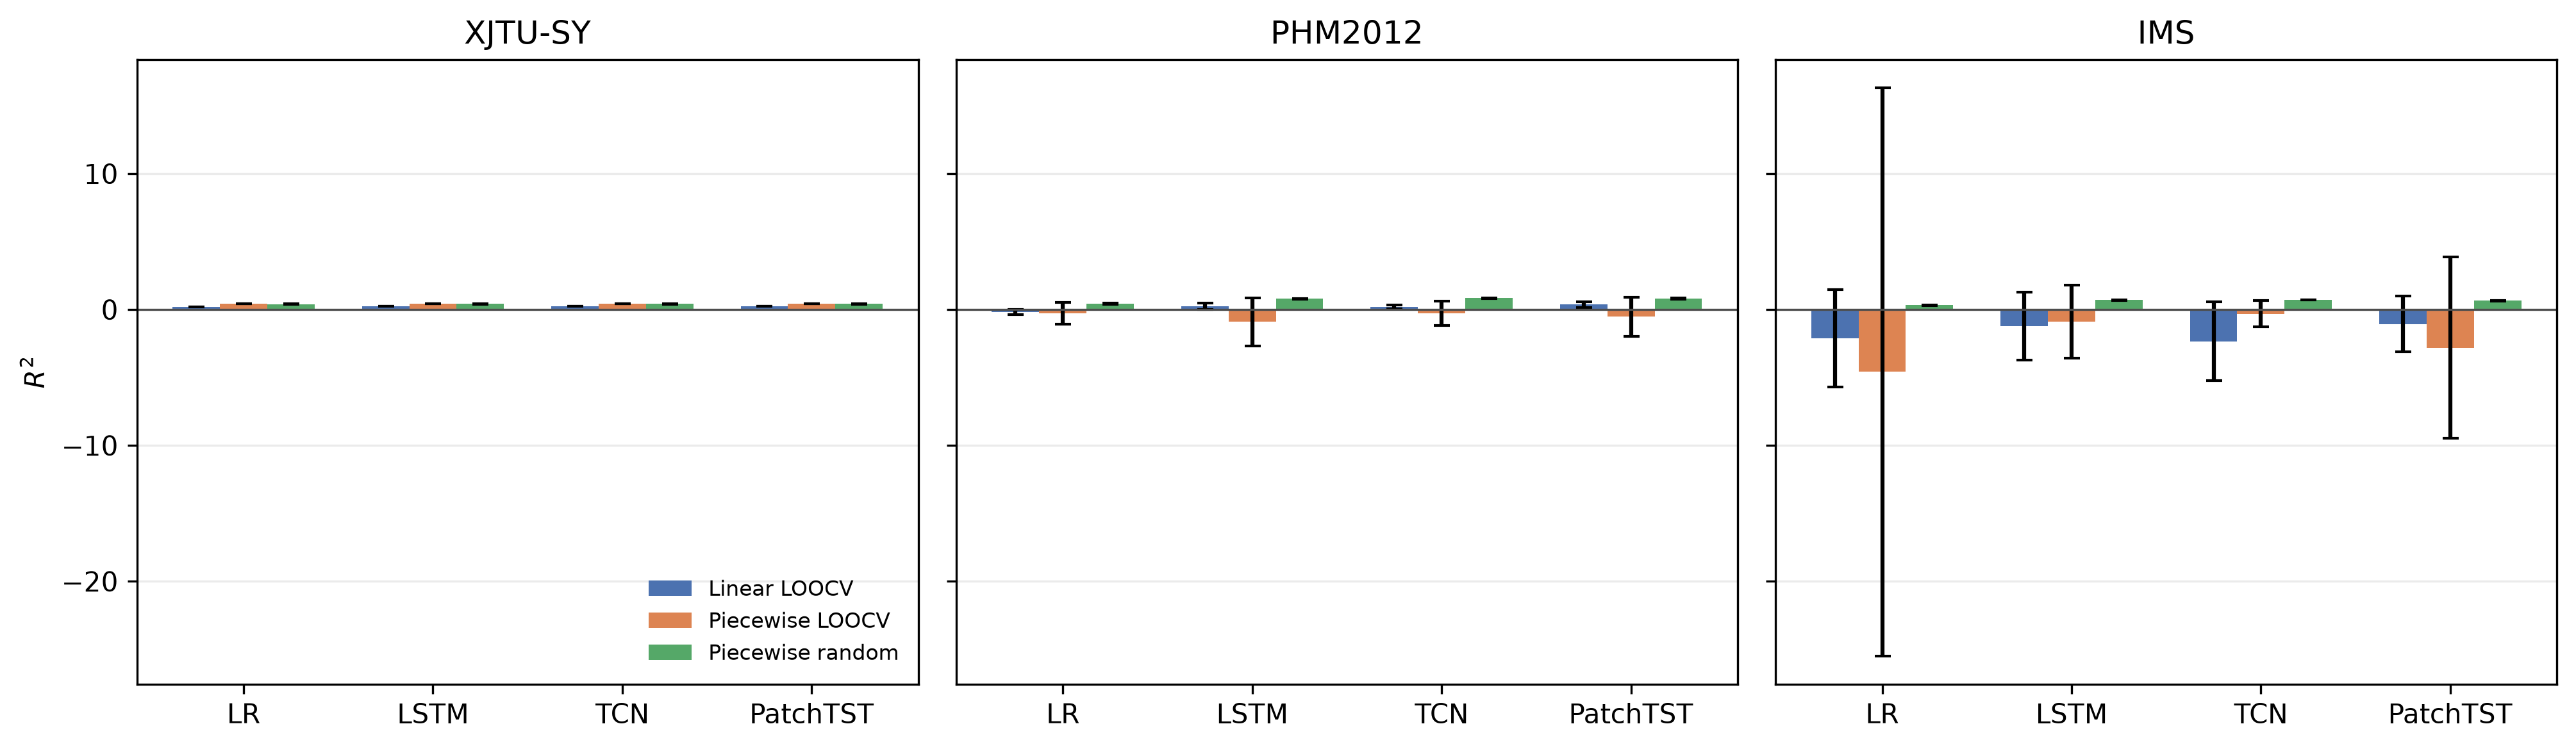
\includegraphics[width=0.48\textwidth]{figures/converged_r2_comparison.png}
\caption{Random time-step splitting consistently raises $R^2$ above linear-LOOCV results, especially on PHM2012 and IMS. Error bars show 95\% confidence intervals for LOOCV and observed min--max ranges for random splits.}
\label{fig:r2}
\end{figure}

\subsection{Constant Baseline and Cross-Bearing Generalization}
The constant predictor has $R^2 \approx 0.000$ on every dataset and label family. Several linear-LOOCV results are below this floor, especially on IMS, where a model must extrapolate across different test rigs and fault modes. This is not a numerical artifact: it shows that cross-bearing generalization is the real challenge. Random time-step splitting hides this failure because test windows come from the same bearings and nearby temporal positions as training windows.

\subsection{Split Sensitivity Results}
Table~\ref{tab:sensitivity} reports TCN results under piecewise labels for the two additional random ratios and the chronological time-block split. The random-ratio results are stable: 60/20/20 and 80/10/10 both remain high, in the same range as the main 70/15/15 result. In contrast, chronological time-block splitting produces large negative $R^2$ on all three datasets. The contrast indicates that the random-split inflation is not an artifact of one particular random ratio; it is consistent with within-trajectory interpolation. The negative chronological results should not be read as a pure leakage effect because temporal extrapolation and degradation-stage imbalance also contribute.

\begin{table}[t]
\centering
\caption{TCN split sensitivity with piecewise labels. Random rows are mean [min--max] over seeds 42, 43, 44; time-block uses chronological 70/15/15 per bearing.}
\label{tab:sensitivity}
\small
\resizebox{\columnwidth}{!}{%
\begin{tabular}{llc}
\toprule
Dataset & Split & $R^2$ \\
\midrule
XJTU-SY & Random 60/20/20 & 0.422 [0.400; 0.436] \\
 & Random 80/10/10 & 0.439 [0.410; 0.458] \\
 & Time-block 70/15/15 & $-4.957$ \\
\midrule
PHM2012 & Random 60/20/20 & 0.857 [0.847; 0.863] \\
 & Random 80/10/10 & 0.879 [0.872; 0.885] \\
 & Time-block 70/15/15 & $-1.812$ \\
\midrule
IMS & Random 60/20/20 & 0.703 [0.698; 0.708] \\
 & Random 80/10/10 & 0.720 [0.716; 0.727] \\
 & Time-block 70/15/15 & $-7.991$ \\
\bottomrule
\end{tabular}}
\end{table}

\subsection{Protocol-Level Reproduction and Its Boundary}
We reproduced the protocol family used by many published high-scoring papers: piecewise 80\% plateau labels, random time-step splitting, converged deep training, and standard statistical features. Under this protocol, deep models reach $R^2$ values of $0.70$--$0.86$ on PHM2012 and IMS, substantially above the linear-LOOCV values.

We do not reproduce $R^2>0.99$. The accurate statement is that the inflation phenomenon is reproducible at the protocol level, but the magnitude in our reproduced protocol family does not reach the near-perfect range reported by some papers. Public code and checkpoints were not available in our environment for the cited papers, so exact reproduction is not possible. We therefore do not claim that all published near-perfect values are explained by evaluation design; our results are consistent with the hypothesis that within-trajectory dependence and interpolation are major contributors.

\section{Discussion}
\subsection{Random Splitting Measures Within-Trajectory Interpolation}
Sliding windows from one bearing are strongly autocorrelated. A random split places test windows from the same trajectory in the training set, so the model can interpolate across almost identical operating phases. Under LOOCV, the test bearing is completely absent during training. The large gaps on PHM2012 and IMS show that the problem is primarily within-trajectory interpolation relative to the intended cross-bearing prediction task, rather than model capacity.

\subsection{Cross-Bearing LOOCV Measures New-Bearing Generalization}
In LOOCV, the held-out test bearing is absent from both training and validation. The protocol therefore answers a different question from random splitting: whether a model can generalize to a bearing whose trajectory has not been observed. Several linear-LOOCV results fall below the constant baseline, especially on IMS. That is not a numerical artifact. It means the model is sometimes worse than predicting the mean when it must leave the training trajectory.

\subsection{Chronological Splitting Measures Temporal Extrapolation}
Chronological splitting keeps the test bearing in training but evaluates later stages of the same trajectory. The negative $R^2$ values in Table~\ref{tab:sensitivity} reflect temporal extrapolation and degradation-stage imbalance as well as the absence of random interleaving. The comparison is still useful because it shows that random splitting, not chronological ordering, is what raises the scores on the same data.

Piecewise labels matter for a second reason: the 80\% plateau makes the label almost constant for most of life. On XJTU-SY, this improves apparent regression performance because the model only needs to recognize the transition region. On PHM2012 and IMS, the plateau can also interact with distribution shift and produce poor LOOCV results. The two practices should be reported separately, not combined into one inflation multiplier.
\subsection{Label Construction Changes Target Difficulty}

Although $R^2$ reflects explained variance, MAE and RMSE quantify absolute prediction deviations. Table~\ref{tab:errors} confirms that the protocol effect is not an artifact of the $R^2$ scale: the piecewise-random protocol consistently reduces RMSE and MAE relative to the linear-LOOCV protocol across all three datasets.

\subsection{Implications for Bearing RUL Benchmarks}
For benchmark reporting, $R^2$ values are not comparable unless the split and label protocols are specified. The complete $2 \times 2$ design in Table~\ref{tab:factorial} separates label, split, and interaction effects more cleanly than a single protocol comparison. MAE and RMSE should accompany $R^2$; a negative $R^2$ under distribution shift can otherwise obscure whether absolute error is actually large.

\subsection{What Does a High $R^2$ Measure?}
A high $R^2$ under random window splitting may indicate interpolation capability rather than cross-bearing predictive ability. The model can rely on adjacent windows from the same trajectory and on the monotonic structure of the label. That kind of performance is useful for tracking a known degradation process, but it does not show that the model can handle a new bearing, a different sensor position, or a different operating regime.

The distinction becomes visible in the LOOCV results. Several models fall below the constant baseline on IMS, which means they are worse than predicting the mean when the test bearing is removed from training. The same models reach much higher $R^2$ under random splitting. The gap is not explained by model capacity. It is explained by the change in what the model is allowed to see.

This interpretation is useful for practitioners. If the deployment task is to monitor a known bearing and detect the transition into late degradation, interpolation-friendly evaluation may be acceptable. If the deployment task is to initialize predictions for a new asset or a new operating condition, benchmark scores must be produced under a cross-bearing protocol. Reporting the protocol is therefore part of reporting what the score means.

\subsection{Practical Reporting Workflow}
A benchmark result is interpretable only when the following items are reported together:
\begin{enumerate}
    \item the intended task, either new-bearing generalization or trajectory tracking;
    \item the split protocol, including whether the test bearing is present in training;
    \item the label construction and all plateau parameters;
    \item the constant or median predictor baseline; and
    \item per-fold results with CI, RMSE, and MAE in addition to $R^2$.
\end{enumerate}
These items are not independent. A random split can inflate $R^2$ even when the model is unchanged, so the split must be reported before the score is interpreted. The same applies to label construction. The STAR template in the next subsection turns this reporting requirement into a reusable checklist.

\subsection{STAR Framework}
We summarize the experimentally supported requirements into the STAR template, which stands for Split integrity, Target integrity, Anchor baseline, and Reporting completeness. In this paper these map to:
\begin{enumerate}
    \item \textbf{Continuous labels}: linear or physics-guided labels as the primary target; plateau parameters must be justified if retained.
    \item \textbf{Leave-one-bearing-out cross-validation}: no training window from the test bearing, with per-fold reporting.
    \item \textbf{Constant predictor baseline}: report the floor below which a model is not informative.
    \item \textbf{Multi-model reporting}: at least two complementary model classes so conclusions are not architecture-specific.
\end{enumerate}
An adaptive debiased label that shortens the plateau and smooths the transition remains a practical intermediate option for applications that need early-stage noise suppression. The current experiments suggest that fixing the split protocol is at least as important as fixing the label.

Table~\ref{tab:star} summarizes the template as an auditable checklist. The checklist is derived from the violations and controls observed in the reproduced protocol family rather than from generic best-practice recommendations.

\begin{table}[t]
\centering
\caption{STAR evaluation template used as an auditable reporting checklist.}
\label{tab:star}
\small
\resizebox{\columnwidth}{!}{%
\begin{tabular}{lll}
\toprule
Component & Minimum requirement & Status in this study \\
\midrule
Split integrity & Test bearing absent from training and validation & Random window split violates; LOOCV satisfies \\
Target integrity & Continuous or explicitly justified label construction & Linear and piecewise labels compared separately \\
Anchor baseline & Constant predictor reported as floor & Included \\
Reporting completeness & Per-fold results, CI, RMSE, MAE, seeds & Included \\
\bottomrule
\end{tabular}}
\end{table}

Table~\ref{tab:star_before_after} shows the contrast between conventional reporting patterns and the STAR requirements. The comparison makes the template actionable: a reader can check each row against a submitted benchmark and see which part of the evaluation protocol is missing.

\begin{table}[t]
\centering
\caption{Conventional reporting patterns versus STAR requirements.}
\label{tab:star_before_after}
\small
\resizebox{\columnwidth}{!}{%
\begin{tabular}{lll}
\toprule
Aspect & Conventional pattern & STAR requirement \\
\midrule
Split & Random window split & Test bearing absent from training and validation \\
Target & Piecewise plateau without justification & Continuous or explicitly justified label \\
Baseline & Constant predictor often omitted & Constant predictor reported \\
Reporting & Final $R^2$ only & Per-fold, CI, RMSE, MAE, seeds \\
\bottomrule
\end{tabular}}
\end{table}

\subsection{Limitations}
We did not reproduce exact published checkpoints because public code was unavailable. IMS has only three held-out test sets, so its confidence intervals are wide; we therefore treat IMS as directional evidence. The external datasets use the same statistical feature pipeline rather than each paper's raw-signal preprocessing. PU is not used because it does not provide run-to-failure trajectories. We do not provide a quantitative prevalence survey in this version; protocol-level claims are limited to the reproduced protocol family. Future work should run exact published pipelines when code becomes available and extend STAR to raw-signal and uncertainty-aware models.

\section{Conclusion}
With converged training on XJTU-SY, PHM2012, and IMS, the combination of piecewise labels and random time-step splitting consistently produces higher $R^2$ than linear-label LOOCV, with Cliff's delta $=1.0$ for the protocol effect in all twelve model-dataset cells. The reproduced protocol family produces $R^2$ values of $0.70$--$0.86$, which are much higher than LOOCV but below the $R^2>0.99$ range reported by some papers. Our results are therefore consistent with the view that evaluation protocol plays a major role in reported RUL performance, while exact near-perfect values still require exact reproduction of the original models and preprocessing. We suggest STAR-style reporting as a possible guideline for future benchmarking so that improvements are measured against a meaningful baseline.

\section*{CRediT Authorship Contribution Statement}
Zhongkuan Ma: Conceptualization, Methodology, Software, Validation, Formal analysis, Writing - Original Draft, Writing - Review \& Editing.

\section*{Declaration of Competing Interest}
The authors declare that they have no known competing financial interests or personal relationships that could have appeared to influence the work reported in this paper.

\section*{Funding}
This research did not receive any specific grant from funding agencies in the public, commercial, or not-for-profit sectors.

\section*{Data and Code Availability}
The XJTU-SY, PHM2012, and IMS datasets are publicly available from their original sources. The reproducibility package is provided as supplementary files and contains preprocessing scripts, converged training and split sensitivity runners, per-fold and per-seed JSON results, table/figure generators, and this manuscript. The code repository is available at \url{https://github.com/KKK-cell441/rul-evaluation-star} and archived at \url{https://doi.org/10.5281/zenodo.21866359}.

\bibliographystyle{elsarticle-num}

\begin{thebibliography}{99}

\bibitem{lei2018machinery}
Y. Lei, N. Li, L. Guo, N. Li, T. Yan, and J. Lin,
``Machinery health prognostics: A systematic review from data acquisition to RUL prediction,''
\textit{Mech. Syst. Signal Process.}, vol.~104, pp.~799--834, 2018.

\bibitem{zhao2019deep}
R. Zhao, R. Yan, Z. Chen, K. Mao, P. Wang, and R. X. Gao,
``Deep learning and its applications to machine health monitoring,''
\textit{Mech. Syst. Signal Process.}, vol.~115, pp.~213--237, 2019.

\bibitem{rul_lstm_uq_2022}
J. Yang, Y. Peng, J. Xie, and P. Wang,
``Remaining useful life prediction method for bearings based on LSTM with uncertainty quantification,''
\textit{Sensors}, vol.~22, no.~12, p.~4549, 2022. doi:10.3390/s22124549.

\bibitem{reg_lstm_2021}
Z.-H. Liu, X.-D. Meng, H.-L. Wei, L. Chen, B.-L. Lu, Z.-H. Wang, and L. Chen,
``A regularized LSTM method for predicting remaining useful life of rolling bearings,''
\textit{Int. J. Autom. Comput.}, vol.~18, no.~4, pp.~581--593, 2021. doi:10.1007/s11633-020-1276-6.

\bibitem{gru_tim_2021}
Z. Que, X. Jin, and Z. Xu,
``Remaining useful life prediction for bearings based on a gated recurrent unit,''
\textit{IEEE Trans. Instrum. Meas.}, vol.~70, pp.~1--11, 2021. doi:10.1109/tim.2021.3054025.

\bibitem{transformer_tim_2023}
H. Peng, B. Jiang, Z. Mao, and S. Liu,
``Local enhancing transformer with temporal convolutional attention mechanism for bearings remaining useful life prediction,''
\textit{IEEE Trans. Instrum. Meas.}, vol.~72, pp.~1--12, 2023. doi:10.1109/tim.2023.3291787.

\bibitem{zhao2021deep}
M. Zhao, M. Kang, B. Tang, and M. Pecht,
``Deep learning for bearing prognostics: A comprehensive review,''
\textit{IEEE Trans. Rel.}, vol.~70, no.~4, pp.~1431--1451, 2021.

\bibitem{caesarendra2021machine}
W. Caesarendra and T. Tjahjowidodo,
``Machine learning methods for bearing fault diagnosis: A comprehensive review,''
\textit{Mech. Syst. Signal Process.}, vol.~152, p.~107397, 2021.

\bibitem{li2022physics}
T. Li, Z. Zhou, S. Li, and Y. Chen,
``Physics-informed neural networks for bearing remaining useful life prediction,''
\textit{Reliab. Eng. Syst. Saf.}, vol.~224, p.~108548, 2022.

\bibitem{ince2016real}
T. Ince, S. Kiranyaz, L. Eren, M. Askar, and M. Gabbouj,
``Real-time motor fault detection by 1-D convolutional neural networks,''
\textit{IEEE Trans. Ind. Electron.}, vol.~63, no.~11, pp.~7067--7075, 2016.

\bibitem{vaswani2017attention}
A. Vaswani, N. Shazeer, N. Parmar, J. Uszkoreit, L. Jones, A. N. Gomez, L. Kaiser, and I. Polosukhin,
``Attention is all you need,''
in \textit{Proc. NeurIPS}, vol.~30, 2017.

\bibitem{paris1963critical}
P. Paris and F. Erdogan,
``A critical analysis of crack propagation laws,''
\textit{J. Basic Eng.}, vol.~85, no.~4, pp.~528--534, 1963.

\bibitem{kotzalas2004fatigue}
M. N. Kotzalas and T. A. Harris,
``Fatigue failure and life prediction of rolling bearings,''
\textit{Tribol. Trans.}, vol.~47, no.~3, pp.~409--418, 2004.

\bibitem{xjtusy2019dataset}
B. Wang, Y. Lei, N. Li, and N. Li,
``XJTU-SY rolling element bearing accelerated life test dataset,''
\textit{Data in Brief}, vol.~25, p.~104122, 2019.

\bibitem{nectoux2012pronostia}
P. Nectoux, R. Gouriveau, K. Medjaher, E. Ramasso, B. Chebel-Morello, N. Zerhouni, and C. Varnier,
``PRONOSTIA: An experimental platform for bearings accelerated degradation tests,''
in \textit{IEEE Int. Conf. Prognostics and Health Management}, 2012, pp.~1--8.

\bibitem{ims2006}
H. Qiu, J. Lee, J. Lin, and G. Yu,
``Wavelet filter-based weak signature detection method and its application on rolling element bearing prognostics,''
\textit{J. Sound Vib.}, vol.~289, no.~4--5, pp.~1066--1090, 2006.

\bibitem{leakage_nature}
N. G. Davies et al.,
``Data leakage jeopardizes ecological applications of machine learning,''
\textit{Nat. Ecol. Evol.}, vol.~7, 2023.

\bibitem{leakage_frontiers}
J. A. Long, J. F. Levesque, and D. L. Huffman,
``Bursting the bubble: Data leakage and inflated deep learning accuracy in multivariate time-series classification,''
\textit{Front. Comput. Sci.}, 2024.

\bibitem{lundberg2017unified}
S. M. Lundberg and S.-I. Lee,
``A unified approach to interpreting model predictions,''
in \textit{Proc. NeurIPS}, vol.~30, 2017.

\bibitem{patchtst2023}
Y. Nie, N. H. Nguyen, P. Sinthong, and J. Kalagnanam,
``A time series is worth 64 words: Long-term forecasting with transformers,''
in \textit{Proc. Int. Conf. Learn. Represent.}, 2023.

\end{thebibliography}

\end{document}
